%%================================================
%% Chapter 2
%%================================================
\chapter{ทฤษฎีหรืองานที่เกี่ยวข้อง}
%\label{literature}
\label{chapter2}

\section{Adobe XD}
\label{Adobe XD}
\begin{figure}[!thb]
	\captionsetup{justification=centering}
	\centering
	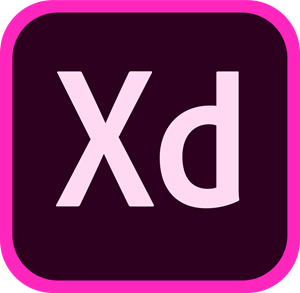
\includegraphics[width=1in]{latex/figures/adobexd.png}
	\captionsource{Adobe XD}{\url{https://www.grappik.com/inside-adobe-xd}}
	\label{fig:adobexd}
\end{figure}
Adobe XD หรือ Adobe Experience Design CC ถูกสร้างมาเพื่อใช้ในการทำงานส่วนของ User Experience Design ไว้ออกแบบ Prototype ได้ทั้งแบบ  Web และ Mobile Application ซึ่งได้รับการพัฒนาและเผยแพร่โดย Adobe Inc สามารถใช้งานได้ทั้งกับ macOS และ Windows มีฟีเจอร์ที่ครบเครื่องทั้งการ ออกแบบ(Design) การเชื่อมประสาน UI (Prototyping) และ การส่งต่องานให้ นักพัฒนา(Developer)
\begin{flushleft}
		\textbf{จุดเด่นของ Adobe XD}
\end{flushleft}
\begin{itemize}
    \item มี Template ให้เลือกและอัปเดตตลอดเวลา ทั้งหน้าเว็บจอ iPhone ไปจนถึงจอ Andriod ทุกขนาด
    \item มีฟังก์ชัน Assets เก็บ Component และ Style ต่าง ๆ ไว้ใช้งานได้รวดเร็ว
    \item สามารถทำ Prototyping จบได้ในโปรแกรม ซึ่งในปัจจุบันการทำ Prototyping เป็นที่นิยมกันมาก เพราะตัว Prototype นั้นสามารถนำไปทดสอบกับ User ได้โดยที่ยังไม่ต้องเขียนโปรแกรม
    \item ในการทำงานสามารถแชร์ให้ลูกค้าดูงานได้แบบ Realtime
    \item มี Plugins มากกว่า 100 ตัวในการช่วยทำงาน
    \item แชร์ไฟล์ทำงานร่วมกับทีมผ่าน Adobe Cloud ในลักษณะ Co-Editing
\end{itemize}
\newpage

\section{Docker}
\label{Dart}
\begin{figure}[!thb]
	\captionsetup{justification=centering}
	\centering
	
\includegraphics[width=2in]{latex/figures/docker.png}
	\captionsource{Docker}{\url{https://medium.com/@rachatatongpagdee/}}
	\label{fig: docker}
\end{figure}
Docker คือ engine ตัวหนึ่งที่มีการทำงานในลักษณะจำลองสภาพแวดล้อมขึ้นมาบนเครื่อง server เพื่อใช้ในการ run service ที่ต้องการ โดยมีลักษณะการทำงานคล้ายคลึงกับ Virtual Machine เช่น VMWare, VirtualBox แต่ข้อแตกต่างที่ชัดเจนคือ Virtual Machine เป็น การจำลองทั้ง OS เพื่อใช้งานและหากต้องการใช้งาน service ใด ๆ จึงทำการติดตั้ง\mbox{เพิ่มเติม} บน OS \mbox{นั้น ๆ} แต่สำหรับ docker แล้วจะใช้ container ในการจำลองสภาพแวดล้อมขึ้นมา เพื่อใช้งาน\mbox{สำหรับ}หนึ่ง service ที่ต้องการใช้งานเท่านั้น โดยไม่ต้องมีส่วนของ OS เข้าไปเกี่ยวข้องเหมือน Virtual Machines อื่น ๆ
\begin{flushleft}
	\textbf{Docker image คืออะไร}
\end{flushleft}
Docker image เป็นเหมือนตัวต้นแบบของ container ซึ่งภายในจะประกอบด้วย application ต่าง ๆ ที่มีการติดตั้งไว้เพื่อใช้งานสำหรับ service นั้น ๆ รวมทั้งมีการ config ค่าต่าง ๆ ไว้เรียบร้อยแล้ว จากนั้นนำมาสร้างเป็น docker image บน registry เพื่อนำไปใช้งาน
\newpage

\begin{flushleft}
	\textbf{จุดเด่นของ Docker}
\end{flushleft}
\begin{itemize}
	\item Docker engine ใช้งานได้บนหลาย platform ทั้งบน Linux, Mac และ Windows
	\item มีขนาดเล็ก สามารถใช้งาน และติดตั้งได้อย่างรวดเร็ว
	\item Docker มีความต้องการในการใช้ CPU, RAM และพื้นที่น้อย
	\item Docker ใช้ทรัพยากรน้อยและเร็วกว่ามาก ไม่ว่าจะเป็น start stop และ restart เพราะใช้ OS, CPU และ RAM ร่วมกันกับ Host OS
	\item Docker มีระบบ Registry ทำให้สามารถเคลื่อนย้าย หรือติดตั้ง Container ได้สะดวก และ\mbox{รวดเร็ว} กว่ามาก
\end{itemize}
\newpage

\section{Visual Studio Code}
\label{Visual Studio Code}
\begin{figure}[!thb]
	\captionsetup{justification=centering}
	\centering
	
\includegraphics[width=2in]{latex/figures/vscode.png}
	\captionsource{Visual Studio Code}{\url{https://medium.com/@vortj/}}
	\label{fig:vscode}
\end{figure}
Visual Studio Code หรือ  VS Code เป็นโปรแกรม  Code Editor ที่ใช้ในการแก้ไขและปรับแต่งโค้ด โดยมาจากค่ายไมโครซอฟต์ มีการพัฒนาออกมาในรูปแบบของ OpenSource เหมาะสำหรับนักพัฒนาโปรแกรมที่ต้องการใช้งานกับแพลตฟอร์มต่าง ๆ ไม่ว่าจะเป็น  Windows, Linux และ macOS   ซัพพอร์ทภาษาหลายร้อยภาษา มีประสิทธิ์ภาพในการใช้งานก็รวดเร็ว รองรับการติดตั้งส่วนเสริม (Plugins) รวมถึงความสามารถในการติดตั้งเครื่องมือเสริม(Extension) ให้เลือกใช้อย่างมาก 

\begin{flushleft}
	\textbf{จุดเด่นของ Virsual Studio Code}
\end{flushleft}
\begin{itemize}
	\item Meet IntelliSense รองรับการใส่สีเพื่อให้อ่านโค้ดง่ายขึ้น (Syntax Highlighting) รวมถึงการคาดเดาที่สิ่ง Dev กำลังจะพิมพ์ (Autocomplete)
	\item Debugging รองรับการ Debug โค้ดภายในตัวโปรแกรมสามารถ Launch โปรเจคขึ้นมาแล้ว debug ด้วย breakpoint, call stacks และที่สำคัญมี Command/Console Prompt ภายในตัว
	\item โปรแกรมสามารถใช้งานได้ฟรี
\end{itemize}
\newpage

\section{Python}
\label{Python}
\begin{figure}[!thb]
	\captionsetup{justification=centering}
	\centering
	
\includegraphics[width=1.5in]{latex/figures/python.png}
	\captionsource{Python}{\url{https://blog.pttexpresso.com/what-is-python/}}
	\label{fig:python}
\end{figure}
ภาษา Python ถูกคิดค้นขึ้นโดย Guido van Rossum โปรแกรมเมอร์ชาวดัตช์ซึ่งมองว่าภาษาโปรแกรมอื่น ๆ  มีความยากและซับซ้อนมากเกินไป จึงสร้างภาษาของตัวเองที่มีความเข้าใจง่ายและทำงานไม่ยุ่งยากขึ้นมา ตัวภาษา Python จะมีความใกล้เคียงกับภาษาอังกฤษมากกว่าภาษา\mbox{โปรแกรม} อื่น ๆ ลดการเรียกใช้ข้อมูลและการใช้ตัวแปรที่ยุ่งยากลง ทำให้ลดบรรทัดในการเขียนได้มาก นอกจากความเข้าถึงง่าย Python ยังมี Library หรือ ตัวช่วยในการใช้งานที่หลากหลาย รองรับตั้งแต่สมการคณิตศาสตร์ วิทยาศาสตร์ จนถึงการจัดการข้อมูลทีเดียว ปัจจุบัน Python เป็น Open Source หรือ ภาษาที่นำมาใช้ได้ฟรีโดยไม่จำเป็นต้องเสียค่าใช้จ่าย ทำให้มีนักพัฒนาจำนวนมากทั้งจากบริษัทเล็ก ๆ  ไปจนถึงบริษัทใหญ่อย่าง Google ให้ความสนใจ และส่งผลให้ตัวของ Python ได้รับการปรับปรุงอยู่เรื่อย ๆ

\begin{flushleft}
	\textbf{จุดเด่นของ Python}
\end{flushleft}
\begin{itemize}
	\item Python เป็นภาษาที่มีความยืดหยุ่นสูงมากและมีฟังก์ชันในการใช้งานมากมาย 
	\item ภาษานี้เป็น Open source ใช้งานได้ฟรี
	\item ง่ายต่อการเรียนรู้ สามารถต่อยอดได้จริง เหมาะสำหรับทั้งผู้เรียนใหม่และคนที่ต้องการต่อยอดจากภาษาอื่น ๆ
	\item มี Tools และ Library Support มาก
	\item มีการใช้งานที่หลากหลาย เมื่อมี Tools และ Library Support มาก ทำให้ในปัจจุบันการ\mbox{ประยุกต์} ใช้งาน Python จึงมีความหลากหลาย ครอบคลุมตั้งแต่การสร้างเว็บไปจนถึงการทำ AI
\end{itemize}
\newpage

\section{Django}
\label{Django}
\begin{figure}[!thb]
	\captionsetup{justification=centering}
	\centering
	
\includegraphics[width=3in]{latex/figures/django.png}
	\captionsource{Django}{\url{https://medium.com/@mitjy/}}
	\label{fig:django}
\end{figure}
Django เป็น framework ที่ใช้ในการสร้าง Web Application ในฝั่งของ Back End ที่พัฒนาด้วยภาษา Python โดยในตัว framework จะมีส่วนประกอบทุกอย่างที่จำเป็นตั้งแต่การเชื่อมต่อฐานข้อมูล ไปจนถึงการ render ข้อมูลออกมาให้ฝั่ง Front End แสดงผลข้อมูลเหล่านั้นได้ ซึ่ง framework ในรูปแบบนี้ในภาษาอื่น ๆ เช่น Ruby on rails สำหรับภาษา Ruby, Play Framework สำหรับภาษา Java หรือ Scala, Groovy on Grails สำหรับภาษา Groovy เป็นต้น

\begin{flushleft}
	\textbf{จุดเด่นของ Django}
\end{flushleft}
\begin{itemize}
	\item มีระบบจัดการ Database ที่ใช้งานง่าย ทำให้จัดการฐานข้อมูลได้เร็วมาก
	\item มีระบบ Admin สำเร็จรูปให้ใช้ เพียงแค่ติดตั้ง Django ก็จะได้รับ Admin 1 ระบบทันที
	\item มีระบบพื้นฐานสำหรับการสร้าง Web Site
	\item Django นั้นเป็น Framework ที่โด่งดัง เลยมีผู้พัฒนาจำนวนมากทำ plugins ที่พร้อมใช้งานเป็นจำนวนมาก
\end{itemize}

